\section{Double Ratchet Algorithm}
\label{ch:dr}
The adoption of a ratchet mechanism is a popular mechanical approach that enables forward movement but inhibits backward movement. A ratchet-like action is performed in the context of secure communication by utilizing randomization in every state update, such that a compromised state is insufficient for the decryption of any subsequent transmission.
The Double Ratchet is a cryptographic asynchronous message exchange algorithm that provides high security to the communicating parties. Asynchronicity in this context refers to that even if the counterpart is not online, the messages should be conveyed (or the key exchange should be done) for a two-party conversation.
Furthermore, a significant design goal dubbed \gls{0rtt} is the ability to transfer payload data without necessitating online exchanges.
\par
The algorithm enables the exchange of encrypted messages based on a shared secret key between the two parties where each message is encrypted with its specific ephemeral key.
The double ratchet algorithm is a combination of two ratchet constructions which provide enhanced security properties.
The first outer ratchet is inherited from \gls{otr}'s asymmetric ratchet to benefit from its future secrecy property which is obtained through the use of ephemeral key exchanges. Coupled by an inner symmetric ratchet for forward secrecy, the algorithm was formed and was formerly named Axolotl Ratchet. Additionally, \gls{kdf} chains are a core concept of the algorithm. This section goes through the methodology of the algorithm, its features, and its security properties.

\subsection{\gls*{kdf} Chain}
As mentioned in section \ref{backgroung:kdf}, a \gls{kdf} is a function that takes as input a key and an input and produces a cryptographically secure hash output that is random-like.
A \gls{kdf} chain is a series of connected \gls{kdf}s where one output key of a \gls{kdf} is a \gls{kdf} key input of a succeeding \gls{kdf}. Figure \ref{fig:kdf-chain} shows an illustration for a \gls{kdf} chain that takes three external inputs and produces three random output keys.

\begin{figure}[hptb]
	\centering
	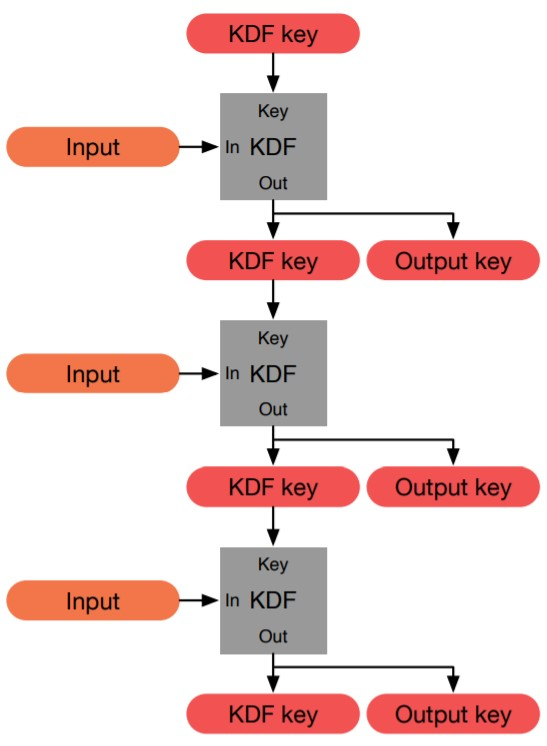
\includegraphics[scale=0.4]{Images/kdf-chain.jpg}
	\caption{A 3 input KDF chain \cite{dblRtcht}.}
	\label{fig:kdf-chain}
\end{figure}

The algorithm session has three \gls{kdf} chains: root chain, sending chain, and receiving chain. Each chain is advanced whenever its relevant ratchet performs a step. More details about ratchet steps and their relation to the \gls{kdf} chains are discussed in later sections.
\par
KDF chains have a set of characteristics \cite{dblRtcht}:
\begin{itemize}
	\item \textit{Resilience:} An adversary who does not know the KDF keys perceives the output keys as random. Even if the opponent has complete control over the KDF inputs, this is still valid.
	
	\item \textit{Forward secrecy:} An adversary who discovers the KDF key at some point in the future cannot distinguish between past output keys and random.
	
	\item \textit{Future secrecy:} If future inputs have contributed adequate randomness, future output keys seem random to an adversary who learns the KDF key at some point in the future.
\end{itemize}

\subsection{Symmetric-key Ratchet}
	
The sending and receiving chains are constructed of symmetric-key ratchets where Alice's sending chain is equivalent to Bob's receiving chain and vise versa. Essentially, a symmetric-key ratchet is a \gls{kdf} chain with a constant input through out the chain steps. However, unlike with random input, a constant input does not provide future secrecy.
\par
In a symmetric-key ratchet, the KDF key illustrated in figure \ref{fig:kdf-chain} is the chain key, while a KDF's output key is a unique message key. For a sending chain, a message key is used to encrypt the outgoing message. On the other side, a message key in the receiving chain is used to decrypt the incoming message. The process of calculating the next chain and message keys is an advance in the sending/receiving chain. This is referred to as a \textit{symmetric ratchet step}.
\par
Message keys are not re-introduced into the KDF chain, therefore, they can be discarded without proposing any security risk to earlier or later ratchet outputs. Also, it is possible to store message keys to handle out-of-order messages on the receiving end. Storing message keys introduce a risk to only their respective messages. However, a compromise of a chain key can lead to further compromise of future chain keys as future chain keys rely on previous ones.

\subsection{Diffie-Hellman Ratchet}
The \gls{dh} ratchet provides the future secrecy property. When paired with the symmetric ratchet, the combination addresses the symmetric ratchet lack of future secrecy. 
Each party generates a \gls{dh} key pair known as their \textit{ratchet key pair}. The parties exchange their public keys within message headers with which each can compute an equivalent \gls{dh} secret output using their own private key that is equivalent to the public key they sent. The process of generating a new \gls{dh} output when receiving a new public key is referred to as a \textit{\gls{dh} ratchet step}. Accordingly, a passive adversary that compromises one party's private key at a point in time is incapable of deducing the upcoming \gls{dh} outputs due to the use of newly generated key pair for each ratchet step.
\par
Next, we discuss an algorithm run where a \gls{dh} ratchet is advanced to create two different DH secret outputs between Alice and Bob. Bob is assumed to be the algorithm initiator. Figure \ref{fig:dh-bobRatchet} serves as visual aid for our discussion where we proceed in steps as labeled in the diagram.

\begin{figure}[hptb]
	\centering
	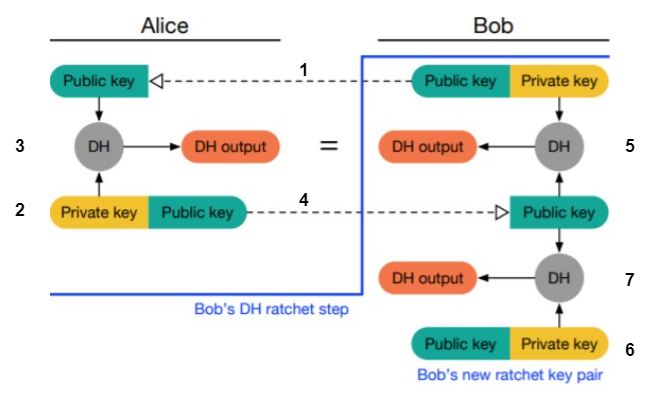
\includegraphics[scale=0.45]{Images/dr-bobRatchet.png}
	\caption{Bob \gls{dh} Ratchet step. Figure reproduced from \cite{dblRtcht}.}
	\label{fig:dh-bobRatchet}
\end{figure}

\begin{itemize}
	\item \textit{Step 1:} Bob generates his first ratchet key pair to send the initial message to Alice. The initial message contains Bob's public key. 
	
	\item \textit{Step 2:} Upon receiving Bob's public key, Alice generates her ratchet key pair.
	
	\item \textit{Step 3:} Alice performs a \gls{dh} calculation between her private key and Bob's public key generating her side of the DH output.
	
	\item \textit{Step 4:} Alice advertises to Bob her public portion of her ratchet key pair that was used to generate the DH output.
	
	\item \textit{Step 5:} After obtaining Alice's ratchet public key, Bob performs a DH calculation between it and his current ratchet private key resulting in Bob's copy of the shared DH output.
	
	\item \textit{Step 6:} Furthermore, Bob generates a new ratchet key pair to generate the next DH output.
	
	\item \textit{Step 7:} Bob performs a \gls{dh} calculation between hit new ratchet private key and Alice's public key generating a new DH output.
\end{itemize}
The steps described above are Bob's DH ratchet step as Bob was the initiator of the ratchet step by advertising his public key. Similarly, Alice's ratchet step starts by sending her public key to Bob and concludes after performing the same steps mentioned above but with the roles reversed.
\par
Linking the algorithm to the messaging context, the DH outputs represent the sending and receiving chains' root keys. 
Each party need to have two chains, sending and receiving chains. Alice's sending chain is equivalent to Bob's receiving chain and vice versa. As depicted in figure \ref{fig:dh-chains}, when a party receives a public key and computes its chain key using a private key that was generated prior to receiving the public, the resulting chain key is the receiving chain key. However, if they private key is generated after receiving the public key, the resulting key is the sending chain key. Simply put, if the public key is used in a DH operation upwards it produces a receiving chain key, while using it in a downwards DH operation generates a sending chain key.
\begin{figure}[hptb]
	\centering
	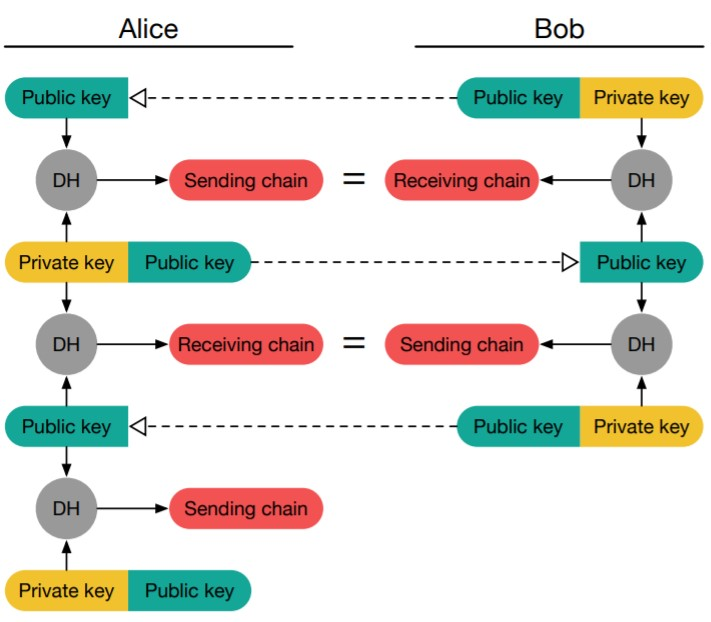
\includegraphics[scale=0.5]{Images/dh-chains.jpg}
	\caption{\gls{dh} chain keys generation \cite{dblRtcht}.}
	\label{fig:dh-chains}
\end{figure}
\par
However, the description so far is simplified. The algorithm is augmented by a KDF chain to improve resilience and future secrecy. The KDF chain key is a shared secret between both parties while the KDF inputs are the DH outputs from the DH ratchet. Every step through the KDF chain results in a new KDF root key and a sending/receiving chain root key. So a full DH ratchet step consists of updating the root KDF chain twice, generating both a sending and a receiving chain key. Figure \ref{fig:dh-ratchet_chain} illustrates a full DH ratchet step.

\begin{figure}[hptb]
	\centering
	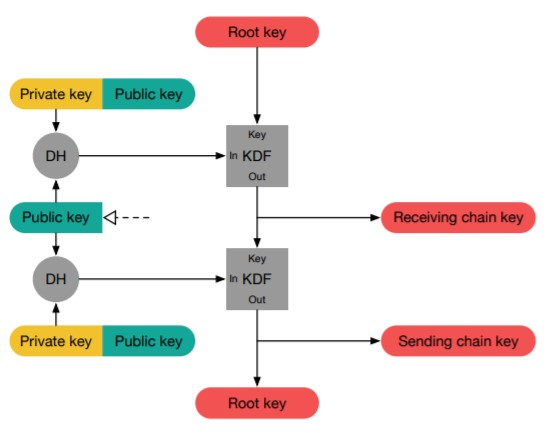
\includegraphics[scale=0.65]{Images/fullDHRatchetStep.jpg}
	\caption{A full \gls{dh} Ratchet step \cite{dblRtcht}.}
	\label{fig:dh-ratchet_chain}
\end{figure}

\subsection{Double Ratchet}
The double ratchet combines both the symmetric-key ratchet and the \gls{dh} ratchet to merge the security advantages provided by each. The outer ratchet is the \gls{dh} ratchet that provides ephemeral DH outputs which improve future secrecy. The DH outputs are fed as inputs to a KDF root chain lying between the outer and inner ratchets. It contributes to augmenting the security features by providing resilience and forward secrecy to the generated keys. The initial \gls{rk} for the KDF chain is a shared secret between the parties, e.g. an output of a key agreement protocol. The KDF chain outputs a new \gls{rk} for the next KDF and a new root \gls{ck} to create a new sending/receiving chain. Lastly the inner ratchet is the symmetric-key ratchet. Their root chain keys are the \gls{ck}s generated from the previous layer. They form the sending and receiving chains. When this ratchet is advanced it generates a new \gls{ck} and a message key. The \gls{ck} is used in the next KDF and the message key is used to encrypt or decrypt the message, depending on its respective chain. 
\par
Figure \ref{fig:AliceDR} serves as an example scenario for an algorithm run as it illustrates Alice's perspective of her double ratchet algorithm after a series of steps. 
\begin{figure}[hptb]
	\centering
	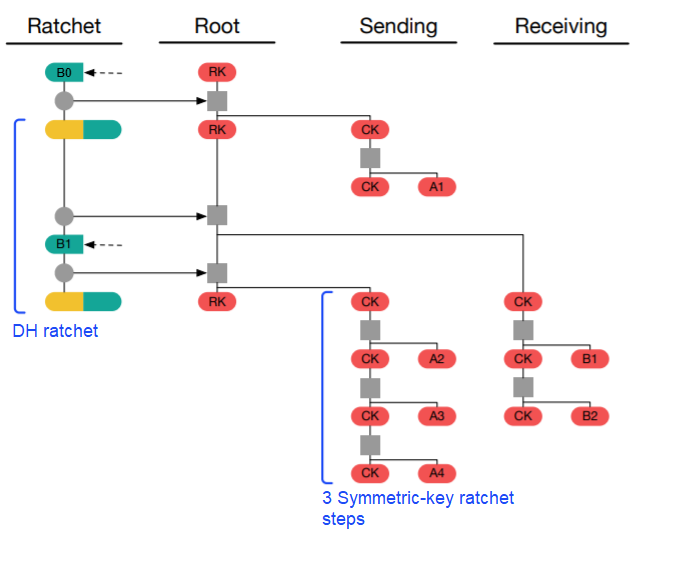
\includegraphics[scale=0.48]{Images/dr.png}
	\caption{Double ratchet from Alice's point of view. Figure reproduced from \cite{dblRtcht}.}
	\label{fig:AliceDR}
\end{figure}
The figure is split into four columns describing the aspects of the algorithm and how they are connected to each other. The first column represents the DH ratchet, the second shows the root KDF chain, and the last two depict the sending and receiving symmetric-key ratchets. Messages are denoted by the initial of the sender and the number of the message, e.g. $A1$ denotes Alice's first message. Keys follow the same abbreviation convention, e.g. $B1$ denotes Bob's first message key. Whether the key is a public key or a message key is represented by their highlighted color. Message keys are highlighted in red while public keys are highlighted in green.
\par
Alice is initialized by receiving the initial public key $B1$ which she uses to compute the input for the root KDF chain through a DH operation. Along with the pre-shared \gls{rk}, Alice computes a root \gls{ck} for her sending chain and a new \gls{rk}. Using the initial \gls{ck}, Alice creates a sending chain by performing a symmetric-key ratchet and producing a new \gls{ck} and a symmetric key $A1$ that she uses to encrypt her first message to Bob.
\par
Till this point, Alice is able to send encrypted messages to Bob as it had created her sending chains. However, she cannot decrypt Bob's messages as she has not yet created a receiving chain to produce the keys required to decrypt Bob's messages. As soon as Bob sends his next message with a new public key, Alice uses the public key $B1$ attached in the message header to step her DH ratchet. $B1$ is used in a DH operation with the previously created key pair to ultimately produce a root \gls{ck} to create a receiving chain. Alice performs a symmetric-key ratchet step of her receiving chain to produce the symmetric key $B1$ that decrypts the received message. Alice advances the same receiving chain to produce message keys to decrypt further message from Bob, e.g. $B2$, as long as the received messages do not contain new public keys in the message headers. However, since Alice received $B1$ and had to perform a full DH ratchet step, she has to generate a new ratchet key pair ultimately create a new sending chain. This implies if Alice wishes to send further encrypted message, she must use the new sending chain to generate the new message key. Thus in figure \ref{fig:AliceDR}, $A2$ is produced from the newly generated sending chain not the old one. As long as Alice has not received a new public key, she keeps advancing the sending chain to generate encryption keys for her outgoing messages, e.g. $A2$ and $A3$ in figure \ref{fig:AliceDR}.
\par
Parties should delete old keys as they no longer have a use. Keys are considered old if they have already been used and they are not going to be used in the future. For example, \gls{rk}s and \gls{ck}s which have already been input into KDFs or message keys that have already been used to encrypt/decrypt messages are considered old keys. Deleting old and useless keys is a good security practice as it prevents intruders from the possibility of recomputing keys that are dependent on those keys. Nevertheless, some keys can be saved to support additional functionalities such as handling out-of-order messages as explained in section \ref{oooMsgs}.

\subsubsection{Out-of-order Messages}\label{oooMsgs}
The Double ratchet algorithm can manage messages arriving out-of-order by simple additions to the message headers from the sender side. By including the message's index $N$ ($N=0$ for message 1) in the sending chain and the length $PN$ of the previous sending chain.
\par
If the sent message does not trigger a DH ratchet step on the receiver side, then the out-of-order message belongs to the current receiving chain of the receiver. The difference between $N$ and the actual receiving chain length is the number steps the receiver has to advance his receiving chain to obtain the message key required to decrypt the received message. The intermediate message keys for the skipped messages are stored in case they arrive later.
\par
On the other hand, if the message triggers a DH ratchet step, then the receiver uses the $PN$ to determine how many messages are skipped of his current receiving chain. The difference between the current length of the chain and $PN$ is the number of steps needed to advanced in the current chains and their produced message keys have to be saved. In this case, $N$ determines the number of skipped messages in the new receiving chain after advancing the DH ratchet. Likewise, the message keys for the skipped messages have to be saved supposing they are delayed for any reason.
\par
Implementation wise, the algorithm defines a \textit{MAX\_SKIP} constant that specifies the maximum number of message keys that should be saved for skipped messages. It should tolerate message loss or delay. However, it should not be too high that it allows for a malicious sender to trigger excessive recipient computation.
\subsubsection{Header Encryption}
As headers contain ratchet public keys as well as $PN$ and $N$ values, a passive attacker can infer the ordering of messages inside a session, or which messages belong to particular sessions. Therefore, encrypting message headers can reinforce messages security. Header encryption is achievable through each party having symmetric keys for both sending and receiving chains to encrypt or decrypt messages' headers. One chain header key is responsible for handling the header encryption of all messages within its respective chain. The header keys are integrated into the double ratchet algorithm as follows.
\par
Originally, Alice and Bob had only one pre-shared secret, the \gls{rk}. To integrate header encryption, the initial shared secrets need to include two unique \glspl{hk}, one for the sending chain and the other for the receiving chain (referred to as \acrfull*{nhk} in \cite{dblRtcht}). The initial \glspl{hk} are used for their respective first generated chains of the algorithm. To continuously obtain new \glspl{hk} for the newly generated chains which are a result of advancing the DH ratchet, the root KDF chain is amended. Instead of generating only a new \gls{rk} and a new respective \gls{ck} with each step, the root chain is modified to additionally produce a \gls{nhk} of the relevant chain. A \gls{nhk} is a \gls{hk} that is to be used for the next chain of the same type that is to be generated after the next ratchet step. In this manner, at any point in time, before generating any chain of the algorithm, there exists already a header key to be used for that chain. When the chain is created, the \gls{nhk} becomes the current \gls{hk} for the chain and a new \gls{nhk} is generated simultaneously for the upcoming chain. Figure \ref{fig:DR-hk} shows an illustration of when \glspl{hk} are generated and how \gls{nhk} are used for the next chains.
\begin{figure}[hptb]
	\centering
	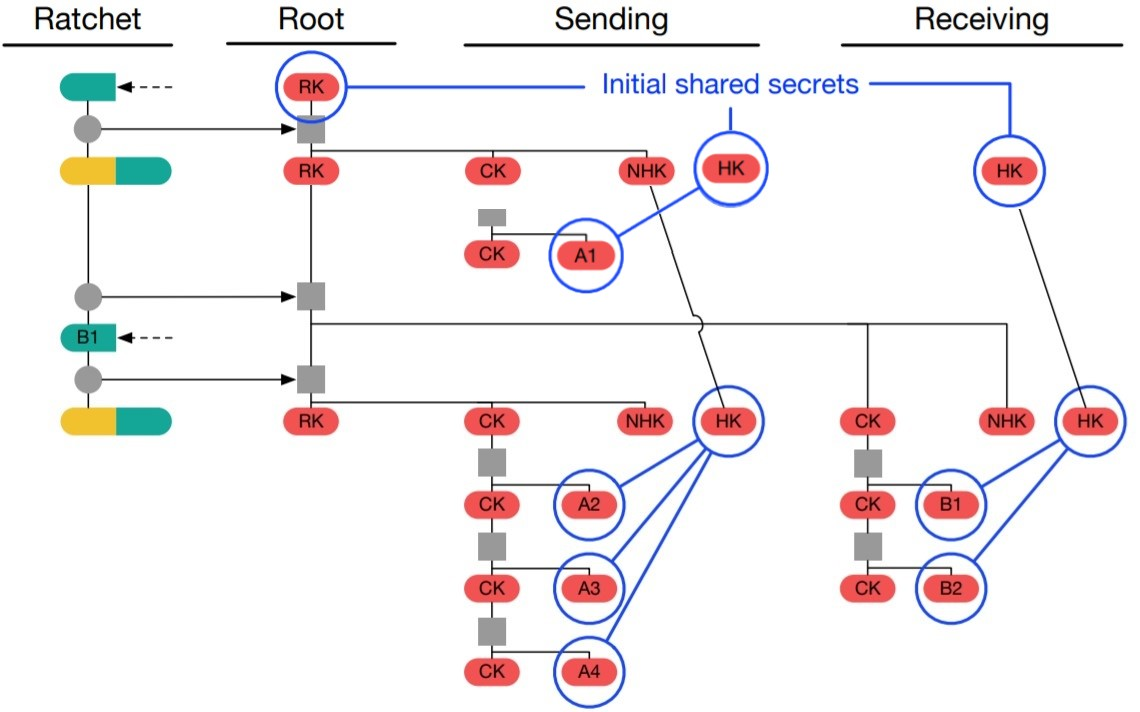
\includegraphics[scale=0.31]{Images/dr-hk.jpg}
	\caption{Usage of \glspl{hk} and \glspl{nhk} in the double ratchet algorithm. Figure reproduced from \cite{dblRtcht}.}
	\label{fig:DR-hk}
\end{figure}